\documentclass[a4paper,12pt]{article}
\usepackage{amsmath}
\usepackage{graphicx}
\usepackage{float}
\title{Computerized Simulation \\
Exercise No. 2}
\author{name : Seyed Mohammad Ghoreishy \\ teacher : Seyed Amirhossein Tabatabaei }
\date{Date: 1403.08.29}
\begin{document}
\maketitle
\tableofcontents 
\newpage

\section{Exercise 1}
Under which condition, the LCG and Multiplicative Congruential methods achieve their maximum period?

\textbf{Solution:}
To achieve the maximum period in the Linear Congruential Generator (LCG) method, the following conditions must be met:
1. The multiplier \( a \) and the modulus \( m \) should be coprime.
2. The increment \( c \) must be coprime with \( m \).
3. The number \( a - 1 \) should be a multiple of all prime factors of \( m \).
4. If \( m \) is divisible by 4, then \( a - 1 \) must also be a multiple of 4.

These conditions ensure that the LCG has the longest possible period before repeating values.

\newline

\section{Exercise 2}
Describe a physical process for generating a sequence of random numbers with 2-digit accuracy.

\textbf{Solution:}
One approach to generate a sequence of random numbers using a physical process is by leveraging thermal noise in an electronic circuit. Thermal noise, caused by the random motion of electrons, is inherently random and can be digitized to produce random numbers. By carefully sampling this noise and rounding it to 2-digit precision, we can achieve a sequence of random numbers with the desired accuracy.

\newpage

\section{Exercise 3}

\begin{figure}[h!]
    \centering
    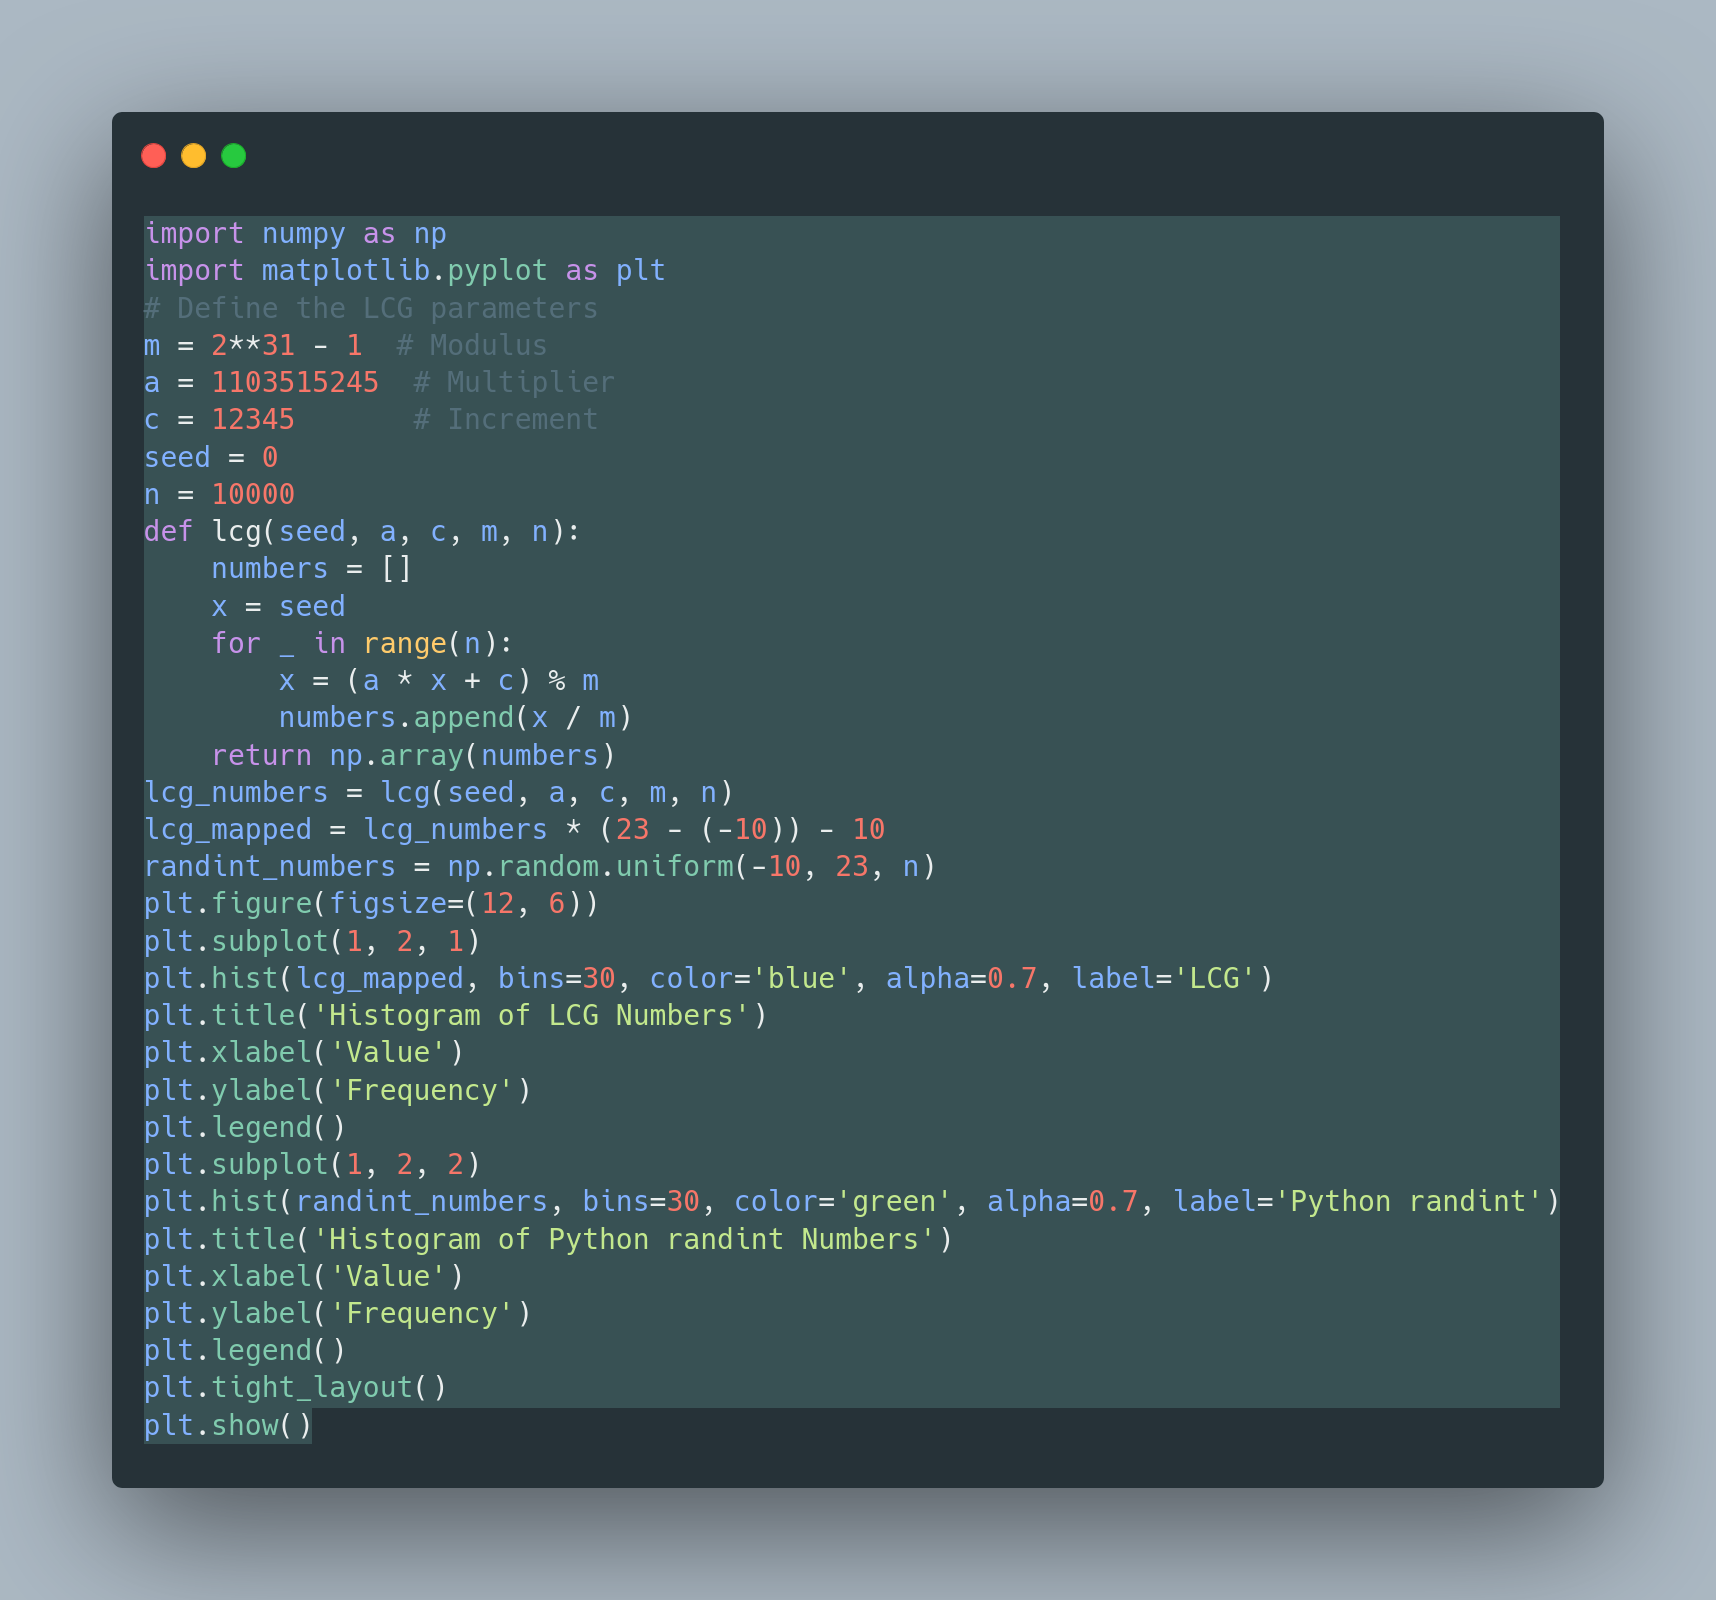
\includegraphics[width=0.6\textwidth]{./Screenshots/3.py.png} 
\end{figure} \\
\begin{figure}[h!]
    \centering
    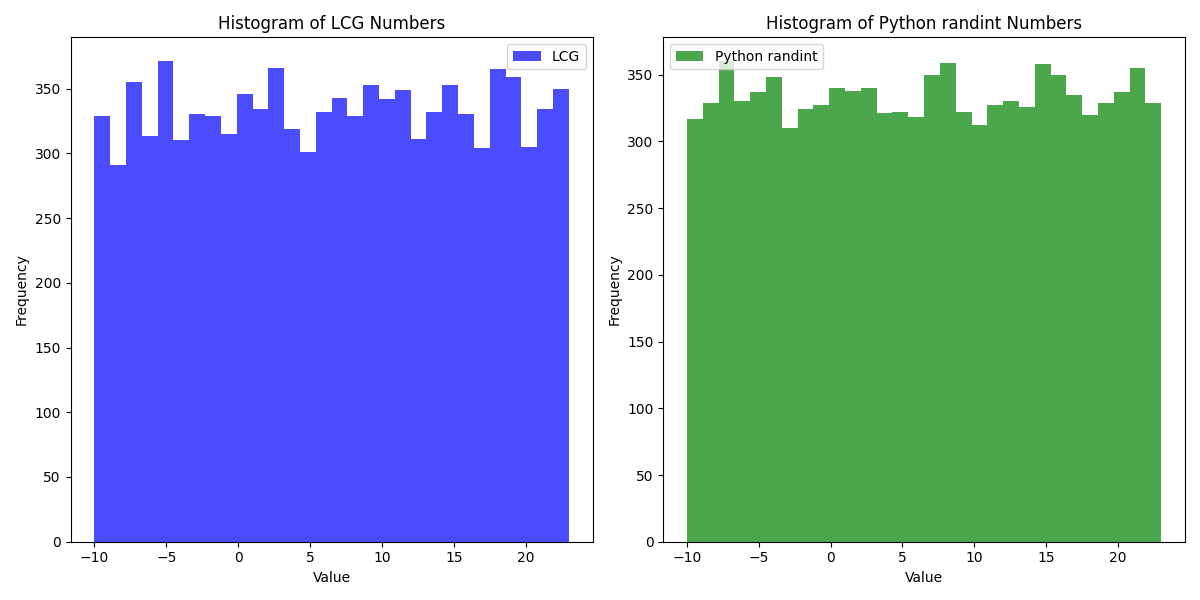
\includegraphics[width=0.6\textwidth]{./Screenshots/3.png} 
\end{figure} 
\newpage

\section{Exercise 4}
just run 4.py and enjoy the output.
\begin{figure}[h!]
    \centering
    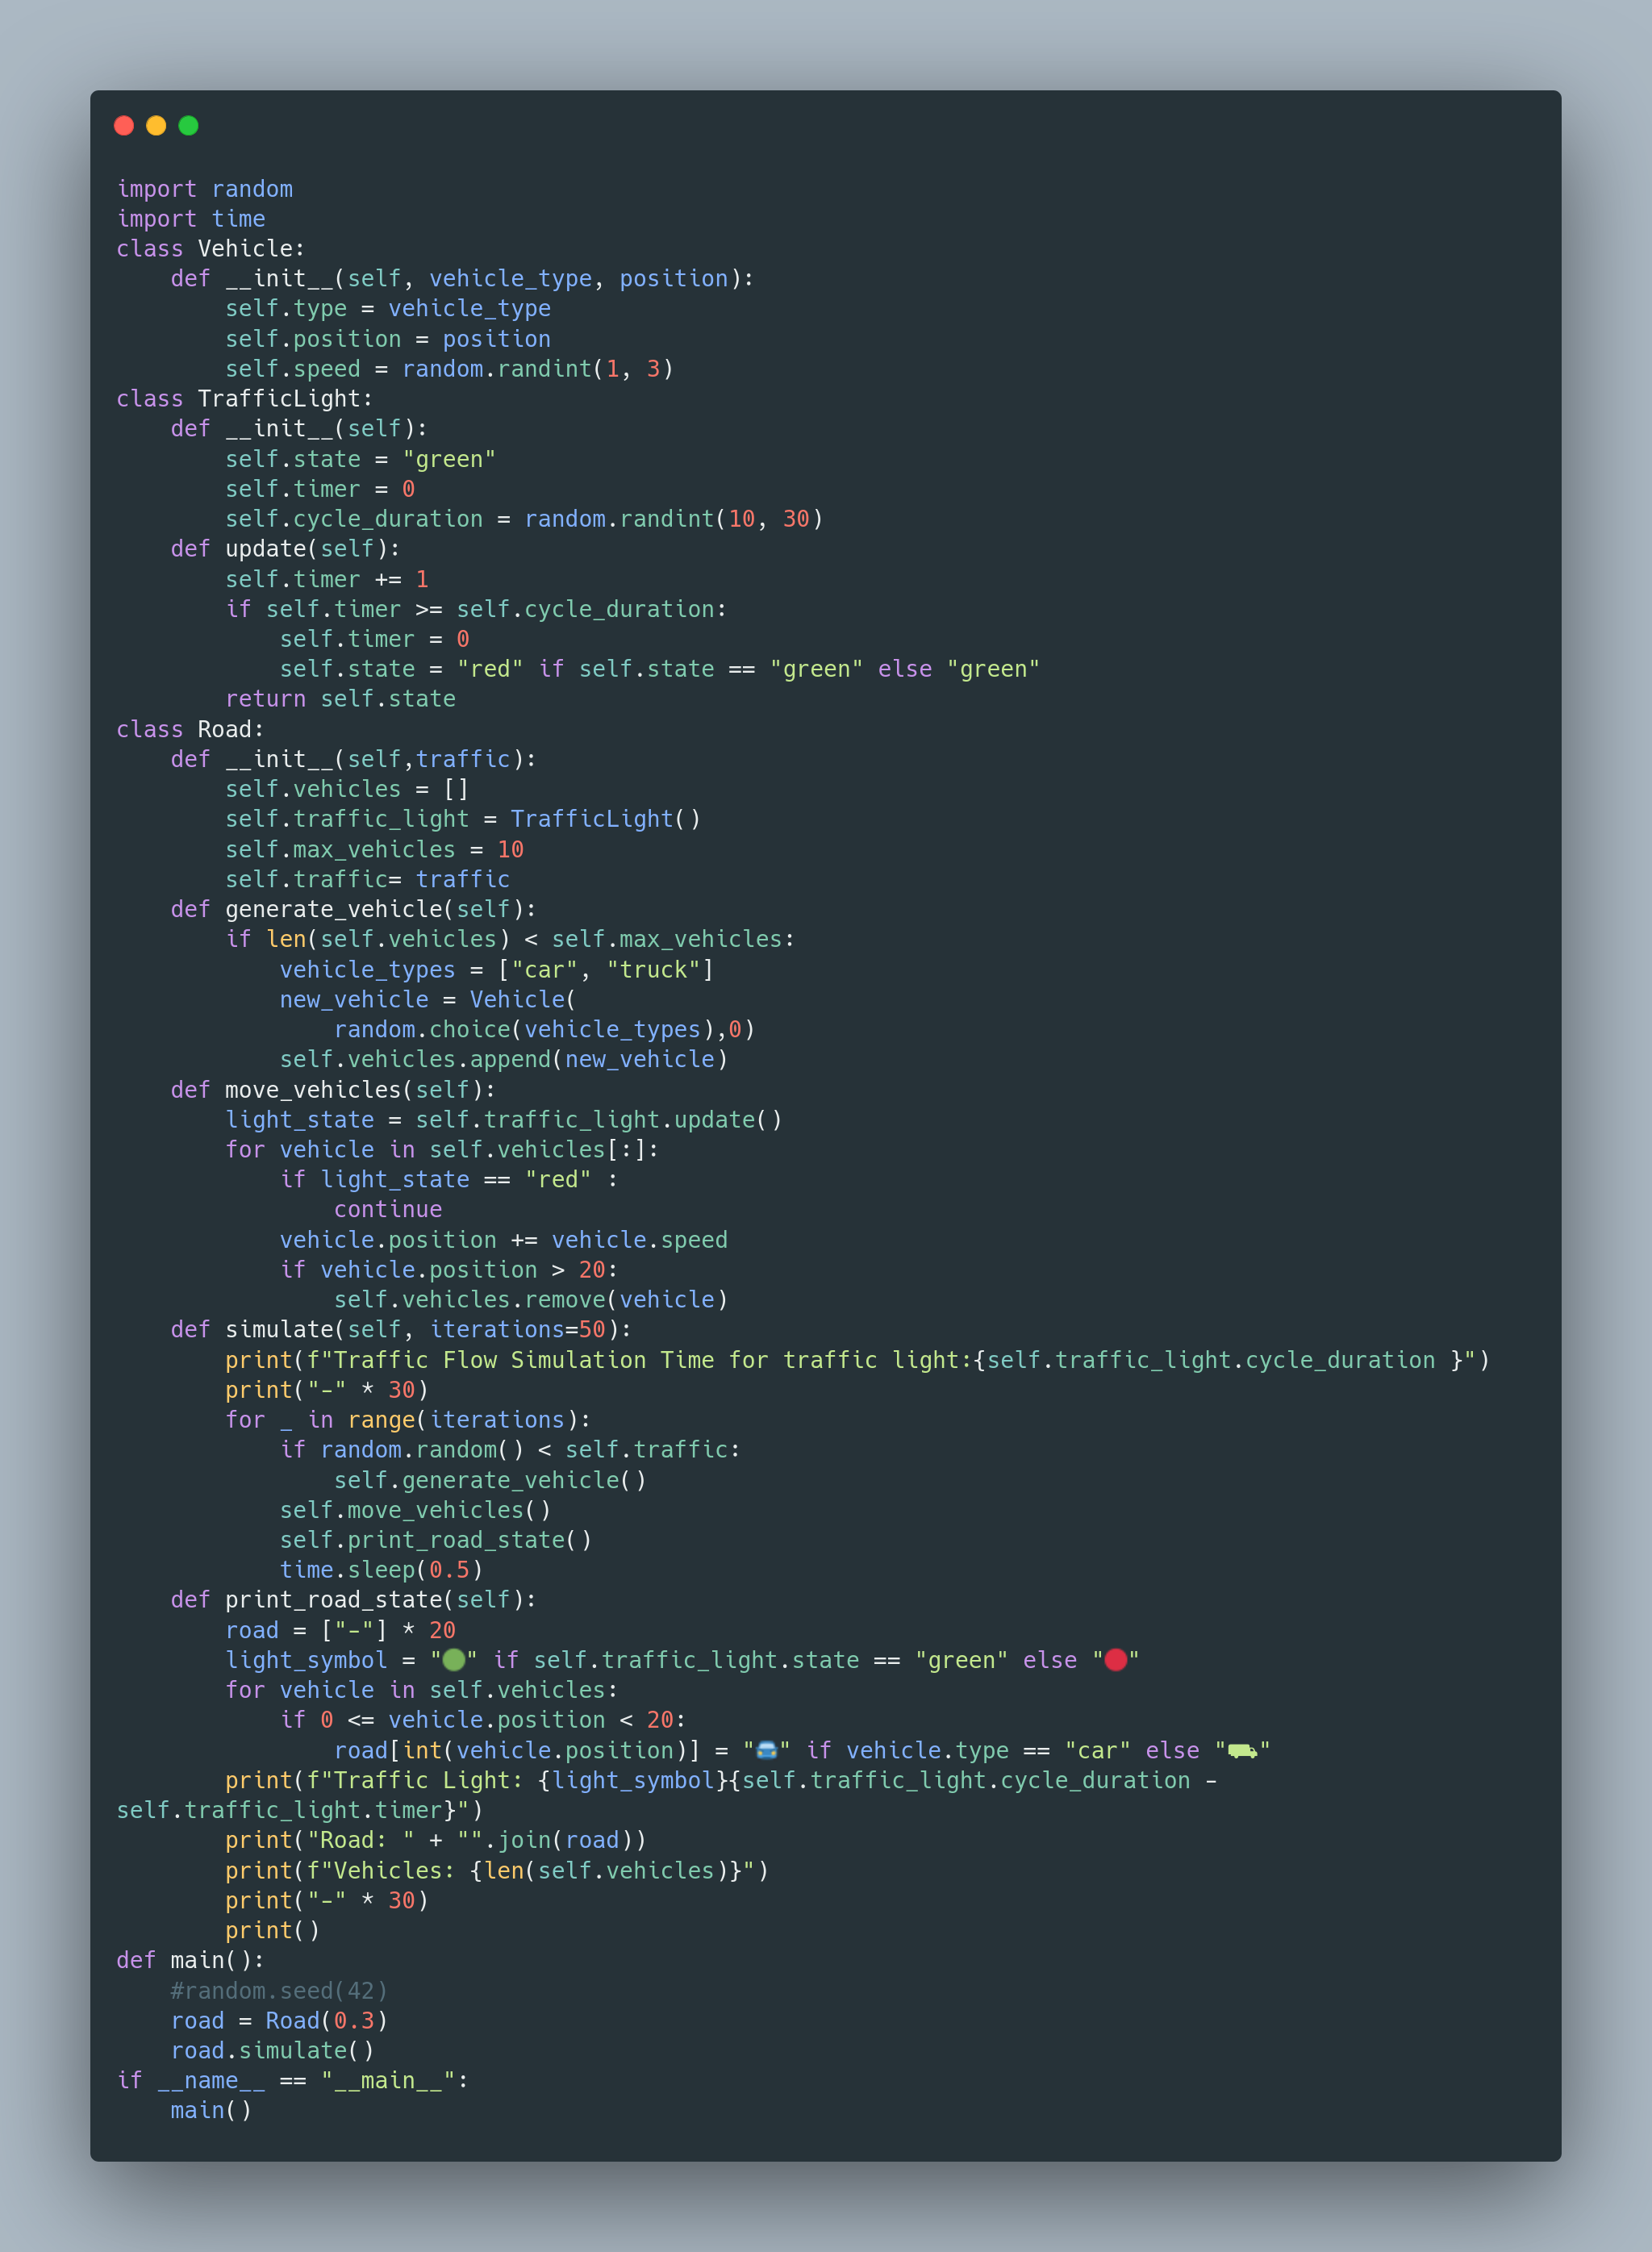
\includegraphics[width=1\textwidth]{./Screenshots/4.py.png} 
\end{figure}
\end{document}
